\documentclass{article}

% Pass 'final' to the neurips_2023 package to remove line numbers if needed
\usepackage[final]{neurips_2023}

% \usepackage[style=authoryear, backend=biber]{biblatex} 
% \addbibresource{main.bib}

\usepackage{graphicx}

\usepackage[utf8]{inputenc} % allow utf-8 input
\usepackage[T1]{fontenc}    % use 8-bit T1 fonts
\usepackage{hyperref}       % hyperlinks
\usepackage{url}            % simple URL typesetting
\usepackage{booktabs}       % professional-quality tables
\usepackage{amsfonts}       % blackboard math symbols
\usepackage{nicefrac}       % compact symbols for 1/2, etc.
\usepackage{microtype}      % microtypography
\usepackage{xcolor}         % colors

\usepackage{hyperref}
\usepackage{cleveref}

\title{Summarization: Contrastive Learning from Exploratory Actions: Leveraging Natural Interactions for Preference Elicitation}

% Paper BibTex
% @inproceedings{dennler2025contrastive,
%   title={Contrastive Learning from Exploratory Actions: Leveraging Natural Interactions for Preference Elicitation},
%   author={Dennler, Nathaniel and Nikolaidis, Stefanos and Matari{\'c}, Maja},
%   booktitle={2025 20th ACM/IEEE International Conference on Human-Robot Interaction (HRI)},
%   pages={778--788},
%   year={2025},
%   organization={IEEE}
% }

\author{
  Summarized by Xiaonan (Nice) Wang \thanks{wangxiaonannice@gmail.com} \\
  % Paper fr last-names (year)
  Summarization\thanks{\textbf{Disclaimer:} This summarization is for research and study purposes. It represents a personal interpretation and may contain inaccuracies. Feedback or corrections via email are highly appreciated.} Generated based on Paper from Dennler, Nikolaidis and Matari{\'c} (2025) \\
  Topic: Human-Robot Interaction, Feature Generation, Preference Learning, Multimodal Learning \\
}

\begin{document}

\maketitle

\begin{abstract}
This document summarizes the core contributions and methodology of the paper "Contrastive Learning from Exploratory Actions: Leveraging Natural Interactions for Preference Elicitation, \cite{dennler2025contrastive}", focusing on its' main ideas and the core blocks.
\end{abstract}

\section{Overview: Core Questions and Answers}

\paragraph{(1) What is the problem?} 
\begin{itemize}
  \item Scenario (the Overall Task): \textbf{Customize} Robot Behaviors that \textbf{Align with Human Preference} -> a.k.a \textit{Preference Learning}
  \item \textit{Low-Dimensional} \textbf{Preference-Aligned (Semantic)} Trajectory \textbf{Features Generation} using Feature Learning Model (a.k.a Feature Generator)
\end{itemize}

\paragraph{(2) Why need to solve this problem?}
\begin{itemize}
  \item Generating semantic human preference-aligned trajectory features when customizing a robot, in order to reduce user interactions for eliciting preferences and improve user satisfaction;
  \item Avoiding data-labelling process like proxy tasks before customizing the robot.
\end{itemize}

% \paragraph{(3) How is it different from prev.?}
% \begin{itemize}
%   \item Hard-Constrained Motion Planner with Proactive Failure Detection and Recovery Mechanism
%   \item Model Agnostic Safety Monitoring Method
%   \item Sim-to-Real Manner for Training Planner Failure Detector
% \end{itemize}


% \paragraph{(4) Why is it better than prev.? (Advantages)} 
% \begin{itemize}
%   \item Advantages among \textit{Typical Hard-Constrained} Methods
%   \begin{itemize}
%     \item Proactive Failure Detection enables \textbf{Adaptability to Disturbances}
%     \item \textbf{Recovery} Mechanism
%     \item Remain Rigor Hard Constrains while Incorporating Failure Processing Strategies (Safety Monitoring+Recovery)
%   \end{itemize}
%   \item Advantages among \textit{Soft-Constrained} Methods
%   \begin{itemize}
%     \item Compliance with Hard Constraints ensures \textbf{Safety}
%     \item Generating Relatively \textbf{Higher Quality} and \textbf{Trackable} Trajectories
%   \end{itemize}
%   \item Advantages among \textit{Reachability Analysis} based Safety Monitoring Methods (Hamilton-Jacobi-Isaacs, ML based, etc.)
%   \begin{itemize}
%     \item \textbf{Generalizability} and \textbf{Model Agnostic}
%   \end{itemize}
%   \item Advantages among Other ML based Failure Detection (Safety Monitoring) Methods
%   \begin{itemize}
%     \item \textbf{More robust}, \textbf{Non-Manual} Recovery Mechanism
%     \item \textbf{Computational Efficient} without Complex DL models
%     \item \textbf{Sim-to-Real} Manner: No Need of Exhaustive Real World Training Data
%   \end{itemize}
% \end{itemize}

% \paragraph{(5) What is the approach itself?}
% \begin{itemize}
%   \item \textbf{Gaussian Process} based \textbf{Proactive Failure Detection} in Motion Planning
%   \item GP-based, sampling-based \textbf{Recovery} after Failure Detection
%   \item \textbf{Sim-to-Real} Training Data for Training Failure Detector
% \end{itemize}

% \begin{figure}[tb]
%   \centering
%   
\includegraphics[width=0.95\textwidth]{fig/gp_robust_motion_planning_diagram.png}
%   \caption{Summarized Block-Diagram of GP-based Robust Motion Planning}
%   \label{fig:gp_motion_planning}
% \end{figure}

% \paragraph{(6) What are the applications of it?} 
% The approach can be demonstrated on several robotic platforms (eg. Boston Dynamics Spot quadruped, Jackal differential drive UGV) for safety-guaranteed and collision-free navigation in unknown environments.

% \section{The Structure}

% \paragraph{Summarized Block-Diagram} 
% The summarized block-diagram see \cref{fig:gp_motion_planning}\footnote{This block-diagram is created through code-based drafting (Graphviz) for efficiency. While visual aesthetics may be limited, the overall structure remains clear.}.

% \paragraph{Original in Paper}

% The original block-diagram see \cref{fig:original}.

% \begin{figure}[tb]
%   \centering
%   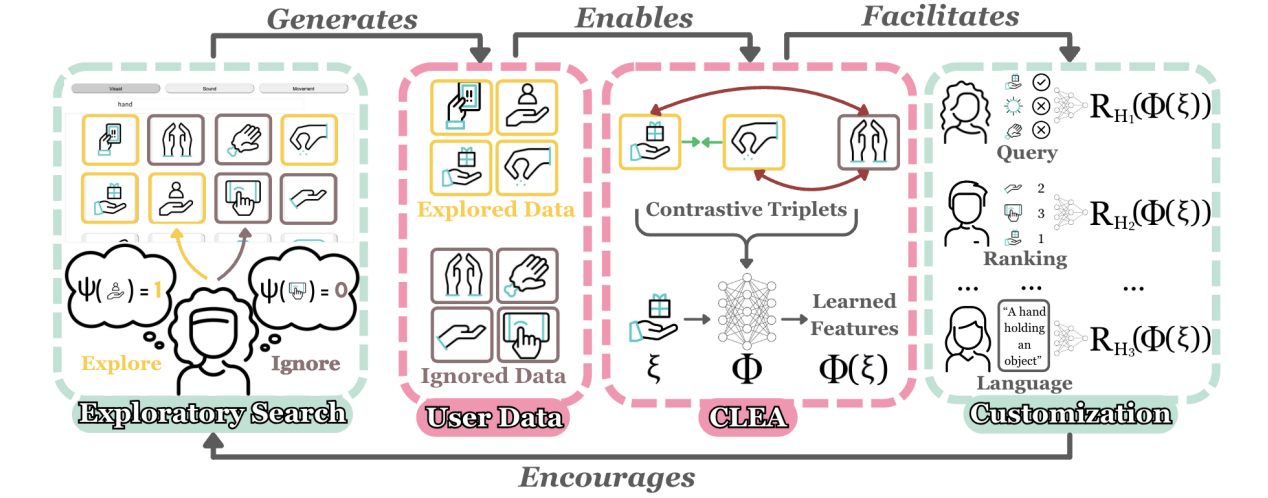
\includegraphics[width=0.95\textwidth]{fig/orig.png}
%   \caption{Original Block-Diagram in Paper}
%   \label{fig:original}
% \end{figure}

% \section{Open Questions}

% \begin{enumerate}
%     \item \textbf{Scalability and Representing Multi-Modal Distributions:} 
%     How does the proposed framework address the $O(N^3)$ computational complexity of Gaussian Processes (GPs) as the robot accumulates more environmental data? Furthermore, can a single Gaussian Process model effectively represent multi-modal failure risk distributions when the true risk landscape exhibits multiple distinct failure modes in topologically complex environments?
%     \item \textbf{Transition to Generative Normalizing Flows:} 
%     Could the current discriminative GP classifier for failure detection be augmented or replaced with a generative Normalizing Flow (NF) model that can capture multi-modal failure risk distributions? Specifically, would NF's latent space representation enable more efficient sampling of recovery candidate states compared to the current sampling approach?
% \end{enumerate}

\bibliographystyle{abbrvnat}
\bibliography{main}
\end{document}
